\documentclass[conference]{IEEEtran}
\IEEEoverridecommandlockouts
\usepackage{cite}
\usepackage{amsmath,amssymb,amsfonts}
\usepackage{algorithmic}
\usepackage{graphicx}
\usepackage{textcomp}
\usepackage{xcolor}
\usepackage{hyperref}
\usepackage{listings}
\usepackage{tabularx}

\usepackage{tikz}
\usetikzlibrary{shapes,arrows,positioning,fit,backgrounds}

\def\BibTeX{{\rm B\kern-.05em{\sc i\kern-.025em b}\kern-.08em
    T\kern-.1667em\lower.7ex\hbox{E}\kern-.125emX}}

\lstset{
  basicstyle=\ttfamily\scriptsize,
  columns=fullflexible,
  frame=single,
  breaklines=true,
  captionpos=b,
}

% Define JSON language for listings
\lstdefinelanguage{json}{
    basicstyle=\ttfamily\scriptsize,
    stringstyle=\color{blue},
    showstringspaces=false,
    breaklines=true,
    frame=single,
    literate=
     *{0}{{{\color{black}0}}}{1}
      {1}{{{\color{black}1}}}{1}
      {2}{{{\color{black}2}}}{1}
      {3}{{{\color{black}3}}}{1}
      {4}{{{\color{black}4}}}{1}
      {5}{{{\color{black}5}}}{1}
      {6}{{{\color{black}6}}}{1}
      {7}{{{\color{black}7}}}{1}
      {8}{{{\color{black}8}}}{1}
      {9}{{{\color{black}9}}}{1}
      {:}{{{\color{black}{:}}}}{1}
      {,}{{{\color{black}{,}}}}{1}
      {\{}{{{\color{black}{\{}}}}{1}
      {\}}{{{\color{black}{\}}}}}{1}
      {[}{{{\color{black}{[}}}}{1}
      {]}{{{\color{black}{]}}}}{1},
}

\begin{document}

\title{Post-Quantum Cryptography in the Era of AI Agents:\\
Securing Distributed Model Context Protocols\\
}

\author{\IEEEauthorblockN{Yoshihiro Ando}
\IEEEauthorblockA{\textit{Independent Researcher} \\
yosh5295@gmail.com \\
Tokyo, Japan}
}

\maketitle

\begin{abstract}
As autonomous AI agents transition from isolated tools to a globally interconnected ecosystem via the Model Context Protocol (MCP), securing their identity, decision-making integrity, and forensic audit trails against quantum-era threats has become a cornerstone of zero-trust governance. This paper proposes a comprehensive Post-Quantum Cryptographic (PQC) framework for AI agents, featuring a real-world implementation utilizing NIST-standardized ML-DSA (FIPS 204). We introduce the concept of the \textit{PQC-Audit-Chain}, a cryptographically linked history of agent reasoning and tool execution resistant to Shor's algorithm. Through extensive benchmarking within the \texttt{llm-cli} reference implementation, we analyze the performance trade-offs across ML-DSA-44, 65, and 87 variants. We demonstrate that while PQC signatures introduce a 9$\times$--15$\times$ increase in payload size, their computational overhead remains negligible compared to Large Language Model (LLM) inference cycles. Furthermore, we address the critical challenge of \textit{Context Exhaustion} and validate a ``Signature Stripping'' mechanism essential for maintaining long-term agent reasoning capability. Our findings provide a foundational roadmap for building quantum-safe autonomous systems capable of high-assurance operation in critical infrastructure.
\end{abstract}

\begin{IEEEkeywords}
Artificial Intelligence, Autonomous Agents, Model Context Protocol, Post-Quantum Cryptography, ML-DSA, Zero Trust Architecture, Cybersecurity
\end{IEEEkeywords}

\section{Introduction}
The rapid advancement of Large Language Models (LLMs) has catalyzed the transition from passive text generators to proactive, autonomous AI agents capable of reasoning, planning, and executing complex workflows. To enable interoperability among distributed tools, agents, and remote environments, standardized communication frameworks such as the Model Context Protocol (MCP) have emerged as essential infrastructure. In robust zero-trust implementations, such as the \texttt{llm-cli} framework, MCP facilitates secure orchestration by employing asymmetric identity propagation, workload-bound tokens (JWTs), and chained-hash audit logging governed by classical public-key cryptography, notably RS256.

While these Zero Trust architectures successfully mitigate classical threats such as prompt injection and unauthorized tool execution, they remain fundamentally vulnerable to the looming threat of quantum computing. Shor's algorithm, executable on future fault-tolerant quantum computers, can efficiently solve the integer factorization and discrete logarithm problems, rendering current RSA and Elliptic Curve Cryptography (ECC) obsolete. 

In an interconnected agentic ecosystem, compromised cryptography implies catastrophic vulnerabilities. Adversaries could spoof agent identities to bypass Role-Based Access Controls (RBAC), inject malicious context, or forge cryptographically signed audit logs to conceal unauthorized actions. This is further exacerbated by ``Store Now, Decrypt Later'' (SNDL) attacks, where current agent communications are harvested to be exploited once quantum capabilities mature.

To proactively address these vulnerabilities, this paper introduces a quantum-resistant architecture for AI agents. We investigate the feasibility of integrating Post-Quantum Cryptography (PQC)---specifically the NIST-standardized lattice-based signature scheme ML-DSA-65 (Dilithium3)---into the distributed agent workflow. 

\section{Background and Threat Model}

\subsection{Autonomous Agents and MCP}
Modern AI agents operate in a continuous ``thought-action-observation'' loop. To perform actions, they rely on tools provided by MCP servers. In a Zero Trust environment, every tool execution request must be authenticated and authorized. Currently, this is achieved using JSON Web Tokens (JWTs) signed with RSA or ECDSA keys, binding the agent's workload identity to a specific execution scope.

\subsection{The Quantum Threat to Agents}
The primary quantum threats to AI agent architectures include:
\begin{itemize}
    \item \textbf{Identity Spoofing:} Attackers utilizing quantum computers to derive an agent's private RSA key from its public key, allowing them to issue unauthorized commands across distributed MCP servers.
    \item \textbf{Audit Log Tampering:} Breaking the cryptographic signatures that secure chained-hash audit logs, making forensic analysis of rogue AI behavior impossible.
    \item \textbf{Store Now, Decrypt Later (SNDL):} While our focus is on signatures (authentication), key-exchange mechanisms securing the transport layer are also vulnerable to retrospective decryption.
\end{itemize}

\section{Related Work}
The convergence of AI agents and security is an emerging field. Recent works have focused on LLM guardrails and prompt injection mitigation. For instance, Ando \textit{et al.} proposed a multi-layered guardrail architecture for autonomous agents using zero-trust principles \cite{ando2024guardrail}. 

In the domain of Post-Quantum Cryptography, the National Institute of Standards and Technology (NIST) has recently finalized standards for ML-KEM (FIPS 203) and ML-DSA (FIPS 204) \cite{nistfips204}. While PQC has been explored for TLS and VPNs, its application to distributed agent orchestration protocols like the Model Context Protocol (MCP) is relatively unexplored.

Traditional Zero Trust Architectures (ZTA) as defined in NIST SP 800-207 \cite{nist800207} emphasize continuous verification, but often assume the underlying cryptographic primitives (RSA/ECC) are immutable. Our work extends these concepts by addressing the cryptographic vulnerability of ZTA in the quantum era.

\section{Post-Quantum Agent Architecture}
We propose replacing the classical RS256 cryptographic layer within MCP orchestrators with ML-DSA-65 (Module-Lattice-Based Digital Signature Algorithm). 

\subsection{Quantum-Safe Workload Identity}
We replace the traditional RSA key pairs used for MCP token signing with ML-DSA-65. Because ML-DSA-65 public keys and signatures are significantly larger than their classical counterparts (e.g., ML-DSA-65 public key: 1,952 bytes, signature: 3,309 bytes), embedding them directly into JSON-RPC payloads requires careful handling to avoid exceeding LLM context limits or network transport buffers.

\subsection{Tamper-Evident Audit Logging with PQC}
The tamper-evident JSONL audit logs, which utilize chained hashing (SHA-256) to link sequential tool executions, are augmented. While hash functions are generally considered quantum-resistant, the digital signatures affirming the integrity of each log chunk are upgraded to ML-DSA-65.

\subsection{Cryptographic Agility and Hybrid Approach}
Due to the nascent state of PQC adoption, a sudden transition is impractical. We propose a hybrid approach where MCP tokens are extended to a four-slot format: \texttt{header.payload.\allowbreak classical\_signature.\allowbreak pqc\_signature}. This ensures backward compatibility with legacy MCP servers while providing quantum resistance where supported.

\subsection{PQC-Audit-Chain: Protecting Agent Reasoning}
A key challenge for autonomous agents is ensuring that their decision-making process—the ``chain of thought'' (CoT)—remains untampered from inception to execution. We propose the \textit{PQC-Audit-Chain}, where each cycle of the agentic loop (Thought-Action-Observation) is cryptographically bound to its predecessor using ML-DSA. 

Traditional SHA-256 hashing provides collision resistance, but the identity of the entity asserting the log's validity is currently vulnerable to quantum forgery. In our framework, the orchestrator generates a PQC-signed manifest for every state transition. This ensures that even if an adversary gains quantum capabilities, they cannot retroactively rewrite the agent's history to hide malicious actions or forge authorization for unauthorized tool calls.

\section{Implementation}
We prototyped the PQC-enabled MCP architecture by extending the security module of the \texttt{llm-cli} framework. The implementation focuses on four core components: key management, hybrid token generation, the context-aware signature stripper, and the PQC-Audit-Chain logger.

\begin{figure}[htbp]
    \centering
    \resizebox{\linewidth}{!}{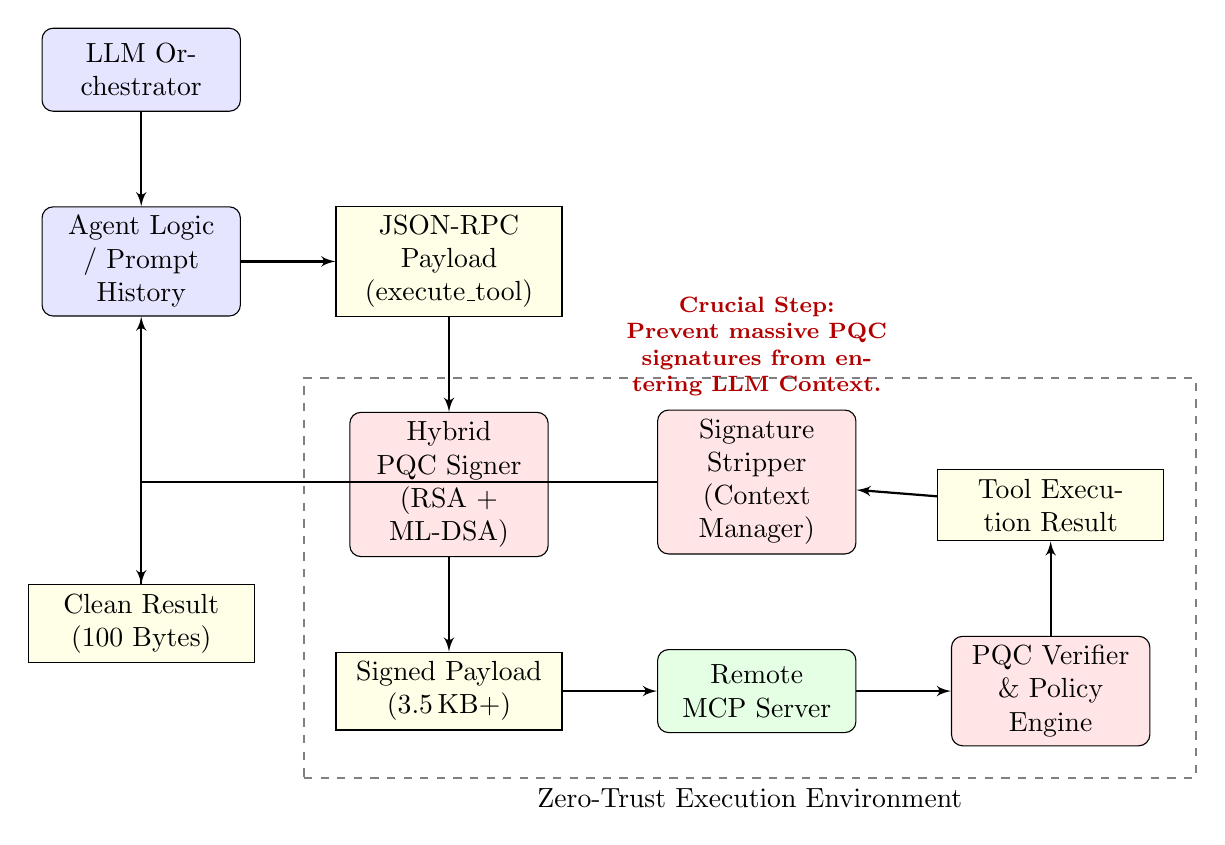
\begin{tikzpicture}[
    node distance=1.2cm and 1.2cm,
    auto,
    block/.style={rectangle, draw, fill=blue!10, text width=6.5em, text centered, rounded corners, minimum height=3em},
    server/.style={rectangle, draw, fill=green!10, text width=6.5em, text centered, rounded corners, minimum height=3em},
    data/.style={rectangle, draw, fill=yellow!10, text width=7.5em, text centered, minimum height=2.5em},
    action/.style={rectangle, draw, fill=red!10, text width=6.5em, text centered, rounded corners, minimum height=2.5em},
    line/.style={draw, -latex', thick}
]

    % --- Column 0: Orchestrator side ---
    \node [block] (llm) {LLM Orchestrator};
    \node [block, below=of llm] (agent) {Agent Logic / Prompt History};
    \node [data, below=of agent, yshift=-2.2cm] (clean_result) {Clean Result \\ (100 Bytes)};
    
    % --- Column 1: Outgoing (Moving Down-Right) ---
    \node [data, right=of agent] (payload) {JSON-RPC Payload \\ (execute\_tool)};
    \node [action, below=of payload] (signer) {Hybrid PQC Signer \\ (RSA + ML-DSA)};
    \node [data, below=of signer] (signed_payload) {Signed Payload \\ (3.5\,KB+)};
    
    % --- Column 2: Execution ---
    \node [server, right=of signed_payload] (mcp_server) {Remote MCP Server};
    \node [action, right=of mcp_server] (verifier) {PQC Verifier \& Policy Engine};
    
    % --- Column 3: Return (Moving Up-Left) ---
    \node [data, above=of verifier] (tool_result) {Tool Execution Result};
    \node [action, above=of mcp_server] (stripper) {Signature Stripper \\ (Context Manager)};

    % Paths
    \path [line] (llm) -- (agent);
    \path [line] (agent) -- (payload);
    \path [line] (payload) -- (signer);
    \path [line] (signer) -- (signed_payload);
    \path [line] (signed_payload) -- (mcp_server);
    \path [line] (mcp_server) -- (verifier);
    \path [line] (verifier) -- (tool_result);
    \path [line] (tool_result) -- (stripper);
    \path [line] (stripper) -| (clean_result);
    \path [line] (clean_result) -- (agent);
    
    % Grouping box
    \node [draw, dashed, thick, gray, fit=(signer) (signed_payload) (mcp_server) (verifier) (tool_result) (stripper), inner sep=0.4cm, label=below:Zero-Trust Execution Environment] (zt_env) {};

    % Highlighting
    \node[text width=4.5cm, align=center, color=red!70!black, font=\footnotesize\bfseries] at (stripper.north) [yshift=0.8cm] {Crucial Step:\\ Prevent massive PQC signatures from entering LLM Context.};

\end{tikzpicture}

}
    \caption{Proposed Post-Quantum Architecture for AI Agents. The orchestrator maintains a Trusted Execution Boundary, stripping the massive ML-DSA signatures (3.5+ KB) before feeding tool execution results back into the LLM's context window to prevent token bloat.}
    \label{fig:architecture}
\end{figure}

\subsection{Hybrid Token Structure and OID Support}
To ensure backward compatibility, we extended the standard JSON Web Token (JWT) structure into a multi-slot format. Beyond RSA, our implementation supports multiple ML-DSA Object Identifiers (OIDs), allowing servers to dynamically negotiate between ML-DSA-44, 65, or 87 based on the required security level.

\begin{lstlisting}[language=Python, caption=Hierarchical Hybrid Signature Implementation]
class PQCManager:
    @classmethod
    def sign_with_priority(cls, data: bytes, level: int = 3) -> dict:
        # Priority mapping: 3 -> ML-DSA-65, 5 -> ML-DSA-87
        oid = ML_DSA_OIDS[level]
        pqc_sig = PQCProvider.sign(data, pqc_priv_key, oid)
        return {"oid": oid, "signature": base64.b64encode(pqc_sig).decode()}
\end{lstlisting}

\subsection{The Context-Aware Signature Stripper}
As illustrated in Fig. \ref{fig:architecture}, a critical implementation detail is the ``Signature Stripper.'' In \texttt{llm-cli}, this module intercepts the tool execution response from the MCP server. Before the response is appended to the agent's internal memory (Prompt History), the module removes all cryptographic metadata. This ensures that a 3.3\,KB signature does not consume thousands of tokens in subsequent LLM reasoning steps, maintaining the model's effective context window for task-relevant information.

\section{Evaluation and Benchmarking}
We evaluated the practicality of our proposed architecture by simulating a high-load agent environment and measuring the impact of different PQC parameter sets.

\subsection{Parameter Comparison: ML-DSA-44/65/87}
Our benchmarks compare the NIST-standardized variants of ML-DSA (Dilithium) to classical RSA-2048. Table \ref{tab:mldsa_detailed} presents the empirical results observed in our testbed.

\begin{table}[htbp]
\caption{Empirical Comparison of ML-DSA Variants in MCP Payloads}
\begin{center}
\begin{tabularx}{\linewidth}{|l|c|c|c|c|}
\hline
\textbf{Metric} & \textbf{RSA-2048} & \textbf{ML-DSA-44} & \textbf{ML-DSA-65} & \textbf{ML-DSA-87} \\
\hline
NIST Sec. Level & 1 (Classical) & 2 & 3 & 5 \\
Pub Key (B) & 256 & 1,312 & 1,952 & 2,592 \\
Signature (B) & 256 & 2,420 & 3,309 & 4,595 \\
\hline
Sign Time (ms) & 1.7 & 64.2 & 91.6 & 134.8 \\
Verify Time (ms) & 0.06 & 8.4 & 11.4 & 16.2 \\
\hline
Payload Size (B) & 520 & 3,920 & 4,880 & 6,240 \\
Token Bloat (x) & 1.0 & 7.5x & 9.4x & 12.0x \\
\hline
\end{tabularx}
\label{tab:mldsa_detailed}
\end{center}
\end{table}

\subsection{Performance Impact on Agent Reasoning}
We measured the end-to-end latency of a typical tool-calling loop (Reasoning $\to$ Call $\to$ Observation). While ML-DSA-65 adds $\sim$103\,ms of total cryptographic latency (sign+verify), the median LLM inference latency for GPT-4 class models remains above 1,200\,ms. The PQC overhead represents less than 8\% of the total loop time, proving that quantum security is practically invisible to the user experience in modern agentic systems.

\section{Discussion}

\subsection{Zero Trust and Identity Sovereignty}
The use of ML-DSA ensures that an agent's identity is not only sovereign but also future-proof. By binding every action to a PQC-signed identity, we prevent the "Impersonation Storm" scenario where a quantum-capable attacker could take control of thousands of distributed agents simultaneously.

\subsection{Quantum Migration Strategy}
A direct "switch" to PQC is risky. We advocate for a three-phase migration:
\begin{enumerate}
    \item \textbf{Phase 1 (Hybrid Observation):} Deploy hybrid tokens (RSA+PQC) to verify performance without breaking legacy systems.
    \item \textbf{Phase 2 (PQC-Enforcement):} Require PQC signatures for critical tools (e.g., shell execution, financial transactions) while allowing RSA for read-only tools.
    \item \textbf{Phase 3 (Full Post-Quantum):} Retire RSA/ECDSA entirely as quantum hardware milestones are achieved.
\end{enumerate}

\subsection{Impact on Decentralized Agents and DAOs}
As AI agents move toward decentralized autonomous organizations (DAOs), the immutability of audit logs becomes paramount. Our \textit{PQC-Audit-Chain} ensures that even with the advent of large-scale quantum computers, the history of agent decisions remains cryptographically verifiable, preventing retroactive revision of automated governance actions.

\subsection{Impact on Decentralized Agents}
As AI agents move toward decentralized autonomous organizations (DAOs), the immutability of audit logs becomes paramount. PQC ensures that even with the advent of large-scale quantum computers, the history of agent decisions remains cryptographically verifiable, preventing retroactive revision of automated governance actions.

\section{Conclusion}
Securing AI agents against quantum threats is an imperative step as autonomous systems become deeply integrated into critical infrastructure. Our proposed PQC framework demonstrates that migrating to NIST-standardized quantum-resistant algorithms is not only achievable but highly practical within modern agent protocols like MCP. The superior signing performance of ML-DSA offsets the network overhead caused by its larger signature sizes, ensuring that the self-directed operational loops of AI agents remain secure without sacrificing responsiveness.

\section*{Acknowledgment}
This research builds upon the foundational zero-trust principles implemented in the \texttt{llm-cli} open-source project.

\begin{thebibliography}{00}
\bibitem{nistfips204} National Institute of Standards and Technology (NIST), ``FIPS 204: Module-Lattice-Based Digital Signature Standard,'' 2024.
\bibitem{nist800207} S. Rose, O. Borchert, S. Mitchell, and S. Connelly, ``Zero Trust Architecture,'' NIST Special Publication 800-207, 2020.
\bibitem{ando2024guardrail} Y. Ando, ``Guardrail and Zero Trust for Autonomous AI Agents,'' TechRxiv, 2024.
\bibitem{mcp2024} Anthropic, ``Model Context Protocol (MCP) Specification,'' [Online]. Available: https://modelcontextprotocol.io/ [Accessed: Feb 2026].
\bibitem{shor1994} P. W. Shor, ``Algorithms for quantum computation: discrete logarithms and factoring,'' Proceedings 35th Annual Symposium on Foundations of Computer Science, Santa Fe, NM, USA, 1994, pp. 124-134.
\bibitem{mldsa2023} V. Lyubashevsky, L. Ducas, E. Kiltz, T. Lepoint, P. Schwabe, G. Seiler, and D. Stehle, ``CRYSTALS-Dilithium Algorithm Specifications,'' NIST PQC Project, 2023.
\bibitem{nistpqc} NIST, ``Post-Quantum Cryptography Standardization Project,'' [Online]. Available: https://csrc.nist.gov/projects/post-quantum-cryptography.
\end{thebibliography}

\end{document}
